\documentclass{article}

\usepackage{fancyhdr}
\usepackage{extramarks}
\usepackage{amsmath}
\usepackage{amsthm}
\usepackage{amsfonts}
\usepackage{amssymb} % Equations
\usepackage{mathtools}
\usepackage{cancel}
\usepackage{commath}
\usepackage{tikz}
\usepackage[plain]{algorithm}
\usepackage{algpseudocode}
\usepackage{adjustbox} % Used to constrain images to a maximum size 
\usepackage{xcolor} % Allow colors to be defined
\usepackage{enumerate} % Needed for markdown enumerations to work
\usepackage{geometry} % Used to adjust the document margins
\usepackage{textcomp} % defines textquotesingle
\usepackage[arrow,matrix,curve,cmtip,ps]{xy}
\usepackage{hyperref}

\usetikzlibrary{automata,positioning}

%
% Basic Document Settings
%

\topmargin=-0.45in
\evensidemargin=0in
\oddsidemargin=0in
\textwidth=6.5in
\textheight=9.0in
\headsep=0.25in

\linespread{1.1}

\pagestyle{fancy}
\lhead{\hmwkAuthorName}
\chead{\hmwkClass\ (\hmwkClassInstructor\ \hmwkClassTime): \hmwkTitle}
\rhead{\firstxmark}
\lfoot{\lastxmark}
\cfoot{\thepage}

\renewcommand\headrulewidth{0.4pt}
\renewcommand\footrulewidth{0.4pt}

\setlength\parindent{0pt}


%
% Create Problem Sections
%

\newcommand{\enterProblemHeader}[1]{
    \nobreak\extramarks{}{Problem \arabic{#1} continued on next page\ldots}\nobreak{}
    \nobreak\extramarks{Problem \arabic{#1} (continued)}{Problem \arabic{#1} continued on next page\ldots}\nobreak{}
}

\newcommand{\exitProblemHeader}[1]{
    \nobreak\extramarks{Problem \arabic{#1} (continued)}{Problem \arabic{#1} continued on next page\ldots}\nobreak{}
    \stepcounter{#1}
    \nobreak\extramarks{Problem \arabic{#1}}{}\nobreak{}
}

\setcounter{secnumdepth}{0}
\newcounter{partCounter}
\newcounter{homeworkProblemCounter}
\setcounter{homeworkProblemCounter}{1}
\nobreak\extramarks{Problem \arabic{homeworkProblemCounter}}{}\nobreak{}

%
% Homework Problem Environment
%
% This environment takes an optional argument. When given, it will adjust the
% problem counter. This is useful for when the problems given for your
% assignment aren't sequential. See the last 3 problems of this template for an
% example.
%
\newenvironment{homeworkProblem}[1][-1]{
    \ifnum#1>0
        \setcounter{homeworkProblemCounter}{#1}
    \fi
    \section{Problem \arabic{homeworkProblemCounter}}
    \setcounter{partCounter}{1}
    \enterProblemHeader{homeworkProblemCounter}
}{
    \exitProblemHeader{homeworkProblemCounter}
}

%
% Homework Details
%   - Title
%   - Due date
%   - Class
%   - Section/Time
%   - Instructor
%   - Author
%

\newcommand{\hmwkTitle}{Homework 02 - Computational}
\newcommand{\hmwkDueDate}{Sept 25, 2018}
\newcommand{\hmwkClass}{Math 6366 Optimization}
\newcommand{\hmwkClassTime}{}
\newcommand{\hmwkClassInstructor}{Andreas Mang}
\newcommand{\hmwkAuthorName}{\textbf{Jonathan Schuba}}

%
% Title Page
%

\title{
    \textmd{\textbf{\hmwkClass:\ \hmwkTitle}}\\
    \normalsize\vspace{0.1in}\small{Due\ on\ \hmwkDueDate}\\
}
\author{\hmwkAuthorName}
\date{}

\renewcommand{\part}[1]{\textbf{\large Part \Alph{partCounter}}\stepcounter{partCounter}\\}

%
% Various Helper Commands
%

% Useful for algorithms
\newcommand{\alg}[1]{\textsc{\bfseries \footnotesize #1}}
% For derivatives
\newcommand{\deriv}[1]{\frac{\mathrm{d}}{\mathrm{d}x} (#1)}
% For partial derivatives
\newcommand{\pderiv}[2]{\frac{\partial}{\partial #1} (#2)}
% Integral dx
\newcommand{\dx}{\mathrm{d}x}
% Alias for the Solution section header
\newcommand{\solution}{\textbf{\large Solution}}


%-------------------------------------------
%       Begin Local Macros
%-------------------------------------------
\newcommand{\Gal}{\mathrm{Gal}}
\newcommand{\Aut}{\mathrm{Aut}}
\newcommand{\Prob}{\mathbf{P}}
\newcommand{\Pow}{\mathcal{P}}
\newcommand{\F}{\mathcal{F}}
\newcommand{\M}{\mathcal{M}}
\newcommand{\A}{\mathcal{A}}
\newcommand{\B}{\mathcal{B}}
\newcommand{\E}{\mathcal{E}}
\newcommand{\n}{\noindent}
\newcommand{\Z}{\mathbb{Z}}
\newcommand{\N}{\mathbb{N}}
\newcommand{\Q}{\mathbb{Q}}
\newcommand{\R}{\mathbb{R}}
\newcommand{\C}{\mathbb{C}}
\newcommand{\T}{\mathbb{T}}
\newcommand{\im}{\operatorname{im}}
\newcommand{\coker}{\operatorname{coker}}
\newcommand{\ind}{\operatorname{ind}}
\newcommand{\rank}{\operatorname{rank}}
\newcommand\mc[1]{\marginpar{\sloppy\protect\footnotesize #1}}
\newcommand{\ra}{\rangle}
\newcommand{\la}{\langle}
%-------------------------------------------
%       end local macros
%-------------------------------------------




\begin{document}

\maketitle


\begin{homeworkProblem}[3]
	Create your own script by extending ex01\_lsq.m to solve the constrained least squares problem given by
	$$\min_x \|	Ax - b\|_2 \ \  \text{subject to}\ x \succeq 0.$$
	Compare your result to the unconstrained case (i.e., plot the solution for both problems in one graph. Submit your script as described in the homework instructions.
	
	\textbf{Solution:}
	
	\begin{figure}[h]
		\centering
		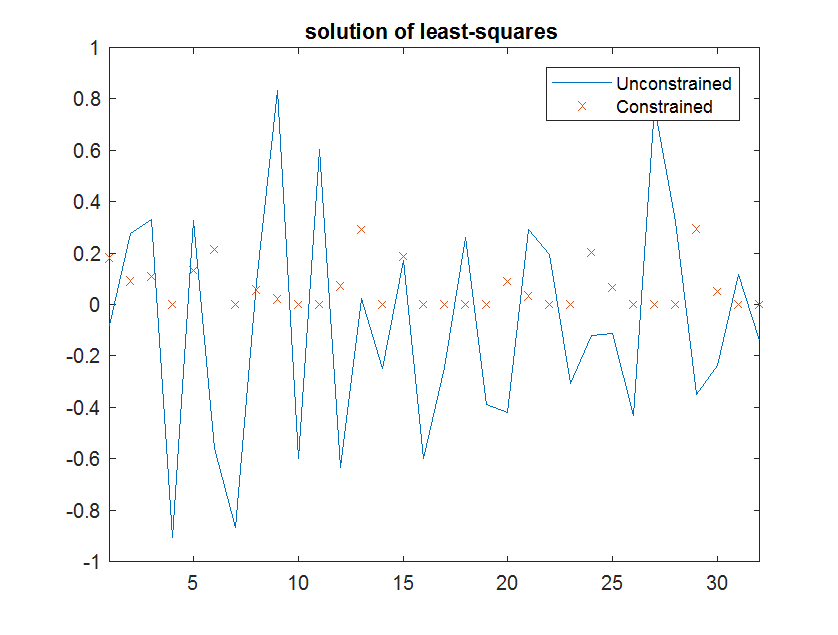
\includegraphics[width=0.7\linewidth]{comp_image/q03}
		\caption{}
		\label{fig:q03}
	\end{figure}
	
	\begin{verbatim}
	# Constrained vs Unconstrained least-squares.
	m = 32; n = 32;
	A = randn(m,n);
	b = randn(m,1);
	
	cvx_begin
	variable x1(n)
	minimize( norm(A*x1 - b, 2) )
	cvx_end
	
	cvx_begin
	variable x2(n)
	x2 >= 0
	minimize( norm(A*x2 - b, 2) )
	cvx_end
	
	figure();
	plot(x1); hold on; plot(x2,'x'); hold off;
	xlim([1,n]);
	legend('Unconstrained', 'Constrained');
	title('solution of least-squares');
	
	\end{verbatim}
	
\end{homeworkProblem}

\begin{homeworkProblem}[4]
	One of the many traps in optimization is working with an erroneous derivative. The following test provides
	a simple way of checking the implementation of a derivative. To this end, let $f$ be a multivariate function
	$f : \R^n \to \R$ and let $v \in \R^n$ be an arbitrary vector in the Taylor expansion
	$$f (x + hv) = f (x) + h\nabla f (x)^\top v + \O(h2).$$
	The vector $g$ is the derivative of f if and only if the difference
	$$| f (x + hv) - f (x) - hg^\top v|$$
	is essentially quadratic in $h$. Implement a derivative check for the least squares problem
	$$	\min_x \frac{1}{2}	\|Ax - b\|^2_2.$$

	Write a general purpose function called checkDerivative that takes a function handle and the vector
	$x$ as input. A common choice for the steps size is h = logspace(-1,-10,10). Notice that you should
	use random vectors to make sure that the derivative check generalizes. The script ex04\_lsq.m illustrates
	some ideas that you might find helpful. For the derivative check, also plot the trend of the error (first and
	second order) versus the step size $h$. Submit a script that runs this derivative check, an implementation
	of the objective function and its derivative, as well as your implementation of the derivative check as
	described in the homework instructions.
	
	
\end{homeworkProblem}

\begin{homeworkProblem}[5]
	Implement a derivative check for the regularized least squares problem
	$$	\min_x \frac{1}{2}	\|Ax - b\|^2_2 + \frac{\beta}{2}\|x\|^2_2.$$
	with regularization parameter $\beta > 0$. Submit a script to run the derivative check, and your implementation
	of the objective function and its derivate as described in the homework instructions.
\end{homeworkProblem}

	\textbf{Solution:}
	
	The solution includes several functions, as follows:
	
	\noindent\rule{\textwidth}{1pt}
	\begin{verbatim}
	% HW02_Question 4 and 5 main
	
	m = 32; n = 32;
	beta = 0.1;
	
	% create random matrices and vectors
	A = randn(n,m);
	b = randn(m,1);
	
	% define function handle for objective
	f = @(x,flag) lsqobj(A,x,b,flag);
	j = @(x,flag) lsqregobj(A,x,b,beta,flag);
	
	x = randn(n,1);
	
	checkDerivative(f, x);
	checkDerivative(j, x);
	\end{verbatim}
	\noindent\rule{\textwidth}{1pt}
	
	The lsqobj function is from the optik package, and helps form a function handle for the least-squares objective function.
	
	\noindent\rule{\textwidth}{1pt}
	\begin{verbatim}
	%######################################################
	% This code is part of the Matlab-based toolbox
	% OPTIK --- Optimization Toolkit
	% For details see https://github.com/andreasmang/optik
	%######################################################
	function [result] = lsqobj(A,x,b,flag)
	% LSQOBJ implementation of objective function for
	% least squares problem
	%
	% inputs:
	%    A         n x m matrix
	%    b         right hand side (vector)
	%    x         current iterate
	%    flag      flag to identify what's going to be computed
	%              options are:
	%              'j'    objective value
	%              'g'    gradient
	%              'h'    hessian
	% outputs:
	%    result    value of objective functional or gradient
	
	switch flag
	    case 'j'
        	% evaluate objective functional j(x) = ||Ax-b||^2_2
        	dr = A*x - b;
        	result = 0.5*dr(:)'*dr(:);
    	case 'g'
        	% evaluate gradient g(x) = A^\T(Ax-b)
        	dr = A*x - b;
        	result = A'*dr;
    	case 'h'
        	% compute hessian A^\T A
        	result = A'*A;
    	otherwise
        	error('flag not defined');	
	end
	end
	\end{verbatim}
	\noindent\rule{\textwidth}{1pt}
	
	The lsqregobj function is modified from above, and helps form a function handle for the regularized least-squares objective function.
	
	\noindent\rule{\textwidth}{1pt}
	\begin{verbatim}
	function [result] = lsqregobj(A,x,b,beta,flag)
	% LSQOBJ implementation of objective function for
	% regularized least squares problem
	%
	% inputs:
	%    A         n x m matrix
	%    b         right hand side (vector)
	%    x         current iterate
	%    beta      regularizer parameter
	%    flag      flag to identify what's going to be computed
	%              options are:
	%              'j'    objective value
	%              'g'    gradient
	%              'h'    hessian
	% outputs:
	%    result    value of objective functional or gradient
	
	switch flag
	    case 'j'
	        % evaluate objective functional j(x) = ||Ax-b||^2_2
	        dr = A*x - b;
	        result = 0.5*dr(:)'*dr(:) + 0.5.*beta.*x'*x;
	    case 'g'
	        % evaluate gradient g(x) = A^\T(Ax-b)
	        dr = A*x - b;
	        result = A'*dr + beta.*x;
	    case 'h'
        	% compute hessian A^\T A
        	result = A'*A + beta.*eye(size(A,2));
    	otherwise
	        error('flag not defined');
	end
	end
	\end{verbatim}
	\noindent\rule{\textwidth}{1pt}
	
	The function checkDerivative evaluates the error in the first order Taylor approximation and plots it.  It evaluates the error in 10 random directions, with increasing distance from the point $x$.  It then plots these 10 error curves, which should all be quadratic.  
	
	\noindent\rule{\textwidth}{1pt}
	\begin{verbatim}
	function [result] = checkDerivative(f, x)
	% Plots the error in the first-order Taylor approximation of 
	% the function f, at x.  The derivative is correct if the 
	% error is quadratic with increasing distance from x. 
	% Plots the error in several random directions.
	
	% inputs:
	%    f          should be a function handle that takes two arguements:
	%               x         current point to evaluate
	%               flag      flag to identify what's going to be computed
	%                           options are:
	%                           'j'    objective value
	%                           'g'    gradient
	%                           'h'    hessian
	
	%    x          current point to evaluate
	% outputs:
	%    result     does nothing
	
	n = length(x);
	num_directions = 10;
	num_steps = 100;
	
	h = logspace(-1, -10, num_steps);
	error = zeros(num_directions,num_steps);
	
	figure(); hold on;
	
	for direction = 1:num_directions
	    v = randn(n,1);
    	for step = 1:num_steps
	        error(direction,step) = abs( f(x+h(step).*v, 'j') - f(x, 'j') - h(step).*f(x, 'g')'*v); 
	    end
	    plot(h, error(direction,:));
	end
	
	title('Absolute error in first-order Taylor approximation');
	xlabel('Distance from point x');
	ylabel('Error');
	result = 0;
	\end{verbatim}
	\noindent\rule{\textwidth}{1pt}
	
	
	\begin{figure}[h]
		\centering
		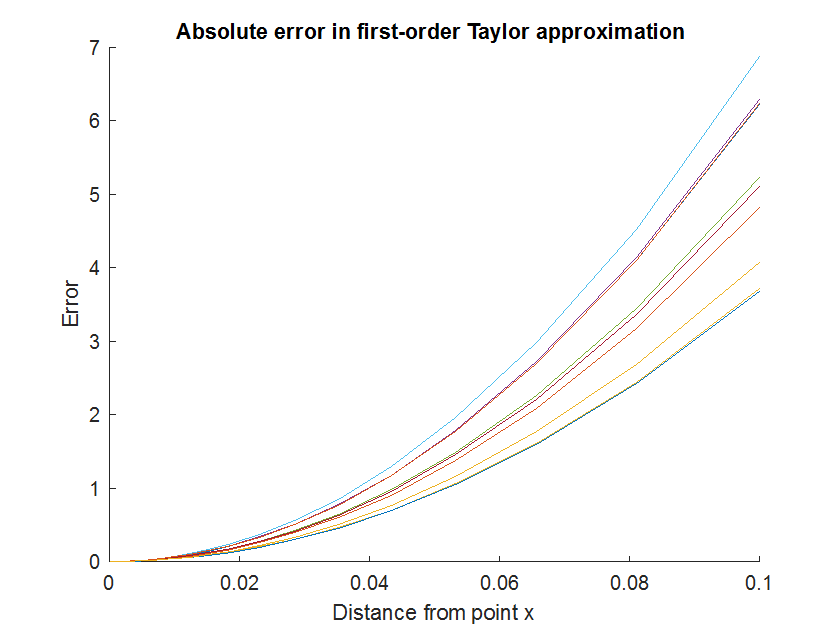
\includegraphics[width=0.7\linewidth]{comp_image/q04}
		\caption[Error for Least Squares problem]{Error for Least Squares problem}
		\label{fig:q04}
	\end{figure}
	
		\begin{figure}[h]
		\centering
		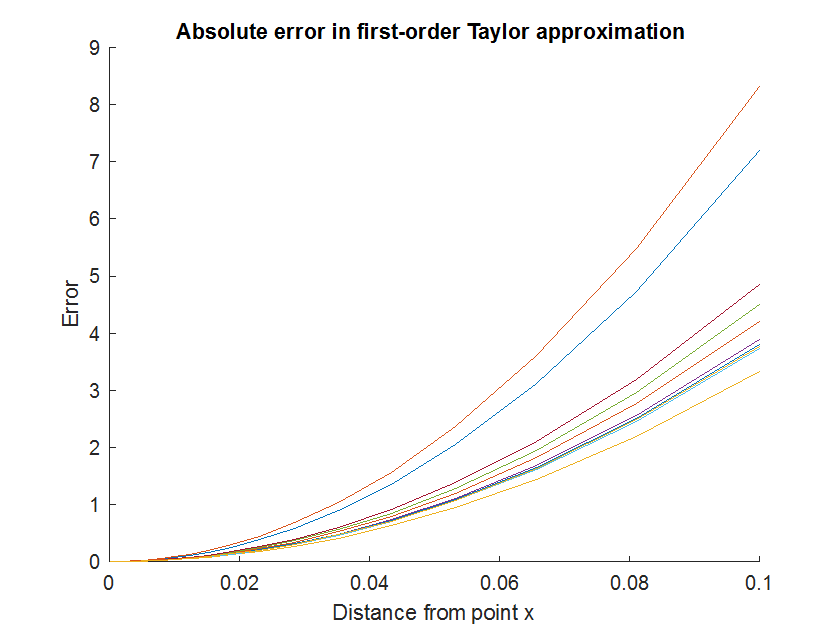
\includegraphics[width=0.7\linewidth]{comp_image/q05}
		\caption[Error for regularized Least Squares problem]{Error for regularized Least Squares problem}
		\label{fig:q05}
	\end{figure}
	
\end{document}